\documentclass[11pt]{scrartcl}
\usepackage[scale=1.5]{ccicons}
\usepackage[notextcomp]{kpfonts} 
\usepackage[margin=1.0in]{geometry}
\usepackage{amsthm,amssymb,amsmath}
\usepackage[pdftex]{graphicx}
\usepackage{subcaption}
\usepackage{enumitem}
\usepackage{bm}
\usepackage{tabu}
\usepackage{mathtools}
\usepackage{tikz}
\usepackage{tikz-3dplot}
\usepackage{xcolor}
\usepackage{colortbl}
\usepackage{wasysym}



\usepackage{color}
\definecolor{darkblue}{rgb}{0, 0, .6}
\definecolor{grey}{rgb}{.7, .7, .7}
\usepackage[breaklinks]{hyperref}
\hypersetup{
	colorlinks=true,
	linkcolor=darkblue,
	anchorcolor=darkblue,
	citecolor=darkblue,
	pagecolor=darkblue,
	urlcolor=darkblue,
	pdftitle={},
	pdfauthor={}
}
\usepackage{fancyhdr}
\thispagestyle{fancy}
\lhead{Math 112-Laird}
\chead{Applications of Exponentials and Logarithms Notes}
\rhead{Spring 2018}
%\lfoot{}%\scriptsize This work is licensed under the \href{http://creativecommons.org/licenses/by-sa/3.0/us/}{Creative Commons Attribution-Share Alike 3.0 License}.} 
%\cfoot{}
%\rfoot{\ccbysa}
\renewcommand{\headrulewidth}{.4pt}
%\renewcommand{\footrulewidth}{.4pt}

\theoremstyle{definition}
\newtheorem{theorem}{Theorem}
\newtheorem*{theorem*}{Theorem}
\newtheorem{acknowledgement}[theorem]{Acknowledgement}
\newtheorem{algorithm}[theorem]{Algorithm}
\newtheorem{axiom}[theorem]{Axiom}
\newtheorem{case}[theorem]{Case}
\newtheorem{claim}[theorem]{Claim}
\newtheorem*{claim*}{Claim}
\newtheorem{conclusion}[theorem]{Conclusion}
\newtheorem{condition}[theorem]{Condition}
\newtheorem{conjecture}[theorem]{Conjecture}
\newtheorem{corollary}[theorem]{Corollary}
\newtheorem{criterion}[theorem]{Criterion}
\newtheorem{definition}[theorem]{Definition}
\newtheorem{example}[theorem]{Example}
\newtheorem{exercise}[theorem]{Exercise}
\newtheorem{journal}[theorem]{Journal}
\newtheorem{lemma}[theorem]{Lemma}
\newtheorem{notation}[theorem]{Notation}
\newtheorem{problem}[theorem]{Problem}
\newtheorem*{problem*}{Problem}
\newtheorem{proposition}[theorem]{Proposition}
\newtheorem{remark}[theorem]{Remark}
%\newtheorem{solution}[theorem]{Solution}
\newtheorem{summary}[theorem]{Summary}
\newtheorem{skeleton}[theorem]{Skeleton Proof}
\newtheorem{activity}[theorem]{Activity}
\newtheorem{intuitivedef}[theorem]{Intuitive Definition}

\DeclareMathOperator{\spn}{span}
\DeclareMathOperator{\Char}{Characteristic}
\DeclareMathOperator{\Aut}{Aut}
\DeclareMathOperator{\stab}{Stab}
\DeclareMathOperator{\Stab}{Stab}
\DeclareMathOperator{\orb}{\mathcal{O}}
\DeclareMathOperator{\lcm}{lcm}
\DeclareMathOperator{\gl}{GL}
\DeclareMathOperator{\Ker}{Ker}
\DeclareMathOperator{\Z}{\mathbb{Z}}
\DeclareMathOperator{\C}{\mathbb{C}}
\DeclareMathOperator{\R}{\mathbb{R}}
\DeclareMathOperator{\N}{\mathbb{N}}
\DeclareMathOperator{\Q}{\mathbb{Q}}
\DeclareMathOperator{\A}{\mathbb{A}}
\DeclareMathOperator{\Gal}{Gal}
\DeclareMathOperator{\PS}{\mathcal{P}}
\DeclareMathOperator{\acc}{acc}


\newenvironment{solution}{\begin{proof}[Solution]}{\end{proof}}
\newcommand{\comment}[1]{%
  \text{\phantom{(#1)}} \tag{#1}
}


%Useful for cut and paste
%\begin{enumerate}[label=\rm{(\alph*)}]

\begin{document}
%%%%%%%%%%%%%%%%%%%%%%% Combining Functions %%%%%%%%%%%%%%%%%%%%%%
%\noindent
%\section*{Warm-Up}
%Complete the following problems:
%\begin{enumerate}
%	\item Calculate the difference quotient $\frac{f(x+h)-f(x)}{h}$ for\\ $f(x)=3x^2+5$. \begin{solution}
%			\textcolor{blue}{First we solve $f(x+h)$, by substituting $x+h$ into $f(x)$ wherever we see an $x$: \begin{align*} f(x+h) &= 3(x+h)^2+5\\ &=3(x^2+2xh+h^2)+5\\ &= 3x^2+6xh+3h^2+5 \end{align*} Next we solve $f(x+h)-f(x)$: \begin{align*} f(x+h)-f(x) &= 3x^2+6xh+3h^2+5- (3x^2+5)\\ &= 3x^2+6xh+3h^2-3x^2-5\\ &= 3h^2+6xh\end{align*} Finally we take the above solution to $f(x+h)-f(x)$ and divide by $h$: \begin{align*} \frac{f(x+h)-f(x)}{h} &= \frac{3h^2+6xh}{h}\\ &= 3h+6x \end{align*} This gives us the final answer of $\frac{f(x+h)-f(x)}{h}=3h+6x$. }
%		\end{solution}
%	\item Transform the following graph via $y=-f(x+2)$ \begin{center}
% 			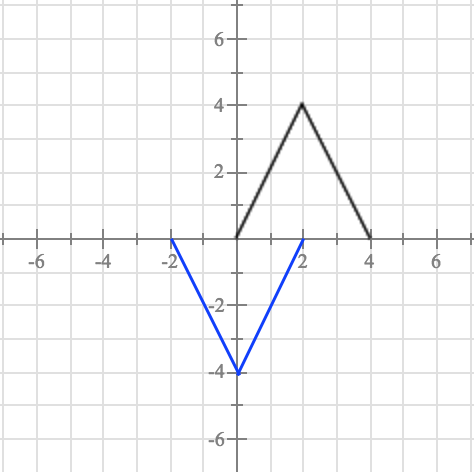
\includegraphics[scale=0.75]{GraphtoTransformSolution}
% 			\begin{solution}
% 				\textcolor{blue}{The original graph is the graph drawn in the black line and the solution is the graph drawn in the blue line. The transformations that were applied was a reflection over the $x$-axis and a horizontal shift left by 2.}
% 			\end{solution}
% 		\end{center}
%
%	\item Graph the following function: \[ g(x)= \begin{cases} -\frac{x}{2} & \text{if } x \neq 2\\ 1 & \text{if } x=2 \end{cases}\] \begin{solution}
%		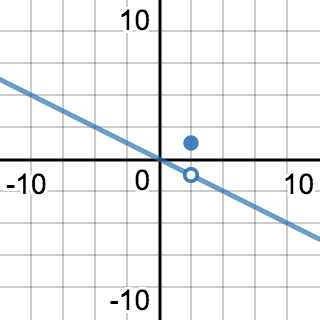
\includegraphics[scale=0.5]{piecewisesolution}
%	\end{solution}
%	
%	\item \textcolor{red}{This is similar to Friday's warm-up} For the following function state the base function and list the transformations in the order in which they were performed. \[f(x)=3\sqrt{-x}+5.\] \begin{solution}
%		\textcolor{blue}{Base Function: $f(x)=\sqrt{x}$\\ Transformations: Reflection over the $y$-axis, vertical stretch by 3, vertical shift up 5.}
%	\end{solution}
%	
%\end{enumerate}
%
%
%\section*{Example 1}
%The local jazz society puts on a series of weekly concerts during the spring. When concert tickets are priced at \$15, the average attendance is 400 people. This past fall the society tried out different ticket prices and found that for every \$2 increase in ticket price, approximately 25 fewer people come to the show. \\
%
%\begin{itemize}
%	\item Write an equation to represent the attendance, $A(x)$, as a function of ticket price $x$.
%	\item Write a function that represents revenue generated by selling tickets as a function of the selling price $x$. 
%	\item When (at what selling price) is revenue maximized?
%\end{itemize}
%
%\section*{Things to know about combining functions}
%\begin{itemize}
%	\item $(f+g)(x)=$
%	\item $(f-g)(x)=$ 
%	\item $(f\cdot g)(x)=$ 
%	\item $\frac{f(x)}{g(x)}=$ 
%	\item $(f \circ g)(x)=$ 
%	\item $(g \circ f)(x)=$ 
%\end{itemize}
%
%\section*{Example 2}
%The sales tax at a certain store is 9\%. 
%\begin{itemize}
%	\item Write a function for the total price paid, $P(x)$, for an item priced at $x$ dollars after factoring in sales tax. 
%	\item The store is having a sale and offering \$5 off every purchase. Write an equation, $S(x)$ for an item originally priced at $x$ dollars.
%	\item Find the composition $P(S(x))$.
%\end{itemize}
%
%\section*{Example 3}
%\begin{enumerate}
%	\item Suppose $h(x)=\frac{3}{\sqrt{x-7}}$. What are two functions $f(x)$ and $g(x)$ such that $(f \circ g)(x)=h(x)$? 
%	\item The following tables show the unemployment rate and crime rates in a certain city. Use these tables to answer some questions.
%		\begin{center}
%			\begin{tabular}{|l|l|}
%\hline
%$t$, time in years & $U$, unemployment rate \\ \hline
%0                  & 0.02                   \\ \hline
%1                  & 0.023                  \\ \hline
%1                  & 0.03                   \\ \hline
%3                  & 0.032                  \\ \hline
%\end{tabular}
%		\end{center} 
%		
%		\begin{center}
%			\begin{tabular}{|l|l|}
%\hline
%$U$, unemployment rate & Crime rate \\ \hline
%0.01                   & 0.015      \\ \hline
%0.02                   & 0.021      \\ \hline
%0.03                   & 0.028      \\ \hline
%0.04                   & 0.031      \\ \hline
%0.05                   & 0.037      \\ \hline
%\end{tabular}
%		\end{center}
%		
%\end{enumerate}

%%%%%%%%%%%%%%%%%%%%%% Inverse Functions %%%%%%%%%%%%%%%%%%%%%%

%\section*{Warm-Up}
%
%Use these functions to answer the following questions: 
%		\[ f(x)=\frac{x}{x-1} \hspace{2cm} g(x)=\frac{4}{x+7}\]
%
%\begin{enumerate}[label=(\alph*)]
%	\item Find $\frac{f}{g}$ \begin{solution}\textcolor{blue}{
%		\begin{align*} \frac{f}{g} &=\frac{\frac{x}{x-1}}{\frac{4}{x+7}}\\ &= \frac{x}{x-1}\cdot \frac{x+7}{4}\\ &=\frac{x(x+7)}{4(x-1)}\\ &= \frac{x^2+7x}{4x-4} \end{align*}
%	}\end{solution}
%	\item What is the domain of $\frac{f}{g}$? \begin{solution}
%		\textcolor{blue}{ The domain of $f$ is $(-\infty, 1) \cup (1, \infty)$, the domain for $g$ is $(-\infty, -7) \cup (-7, \infty)$. The domain of $\frac{f}{g}$ is the intersection of the domain of the two and the ``bad" points for the new denominator. In this case, $(-\infty, -7) \cup (-7,1) \cup (1, \infty)$. }
%	\end{solution}
%\end{enumerate}		
%
%\section*{Introductory Example}
%Suppose that the demand for a certain pair of sunglasses can be expresses as a function of the purchase price using the equation $q=f(p)= -4000p+200,000$. Use this equation to answer these questions:
%\begin{enumerate}[label=(\alph*)]
%	\item What is the demand when the price is \$40? 
%	\item What is $f(0)$ and what does this mean in practical terms? 
%	\item Graph this function in a reasonable window. 
%	\item What are the domain and range of this function? 
%	\item What price corresponds to a demand of 80,000 pairs of sunglasses? 
%\end{enumerate}
%
%
%\noindent
%\section*{Things you need to know about inverse functions}
%When does a function have an inverse function?\\ %\textit{A function is invertible if it is one-to-one, every output variable has exactly one input variable. Graphically it must pass the horizontal line test}
%
%\noindent
%How do you find an inverse function, for a function that has one?\\ %\textit{Solve for the input variable as a function of the output variable}
%
%\noindent
%Notation:\\ %\textit{If $y=f(x)$, then the inverse is denoted $x=f^{-1}(y)$}
%
%\noindent
%Domain/Range: \\ %\textit{The domain of $f^{-1}$ is the range of $f$. The range of $f^{-1}$ is the domain of $f$}
%
%\noindent
%\section*{Practice Example}
%Find the inverse function and evaluate $f^{-1}(57)$ for the following function: \[y=f(x)=7x^3+1\]
%
%\section*{Does an inverse exist?}
%Below is a verbal description of several functions. Determine whether the function described has an inverse function, and if it does, explain what the inverse function tells you.
%\begin{itemize}
%	\item $T=f(p)$ represents the city sales tax paid on an item that sells for $p$ dollars %\textit{If you know an amount of tax, can you (uniquely) determine the price of the item?}
%	\item $C=f(t)$ represents the average cost of a gallon of unleaded gasoline in Tucson $t$ days after January 1 %\textit{If you know an average price of gas, can you (uniquely) determine the price of the item?}
%	\item The profit function $P(x)$, found from the revenue function $R(x)=x\left( \frac{100,000-x}{2000}\right)$ and the cost function $C(x)=1200+10x$, where $x$ is the number of units sold %\textit{Graph and use the horizontal line test}
%\end{itemize}
%
%\section*{Example}
%Suppose a cost-benefit model is given by $C=f(x)=\frac{6.6}{100-x}$ where $C$ is the cost, in thousands of dollars, of removing $x$ percent of a given pollutant. Find the inverse function, and explain what it represents.
%
%\section*{Concept Check}
%The functions $u$ and $w$ are defined as follows: \[ u(x)=-x-2\] \[v(x)=2x^2+1\] 
%\begin{enumerate}
%	\item Find $u(v(-2))$. \begin{solution}
%		\textcolor{blue}{$v(2)=2(-2)^2+1=9$\\ $u(v(-2))=u(9)=-9-2=-11$}
%	\end{solution}
%	\item Find $v(u(x))$.\begin{solution}
%		\textcolor{blue}{\begin{align*}
%			v(u(x))&=2(-x-2)^2+1\\ &= 2(x^2+4x+4)+1\\ &= 2x^2+8x+8+1\\ &= 2x^2+8x+9
%		\end{align*}}
%	\end{solution}
%	\item Find $(u+v)(1)$. \begin{solution}
%		\textcolor{blue}{$u(1)=-1-2=-3$,\\ $v(1)=2(1)^2+1=2+1=3$,\\ so $(u+v)(1)=u(1)+v(1)=-3+3=0$}
%	\end{solution}
%\end{enumerate}
%
%%%%%%%%%%%%%%%%%%%%%%% Day 17 Handouts %%%%%%%%%%%%%%%%%%%%%%
%
%\section*{Warm-Up}
%\begin{enumerate}
%	\item Suppose the functions $g$ and $h$ are defined as follows: \[ g(x)=\frac{8}{x}, x \neq 0 \] \[ h(x)=x^2-7\] Find the compositions $g \circ g$ and $h \circ h$. \begin{solution} \textcolor{blue}{\begin{align*}
%		g \circ g &= \frac{\frac{8}{x}}{\frac{8}{x}}\\ &= \frac{8}{x} \cdot \frac{x}{8}\\ &= \frac{8x}{8x}\\ &=1
%	\end{align*} \begin{align*}
%		h \circ h &= (x^2-7)^2-7\\ &= x^4-14x^2+49-7\\ &= x^4-14x+42
%	\end{align*}} \end{solution}
%	\item \textcolor{white}{a}\\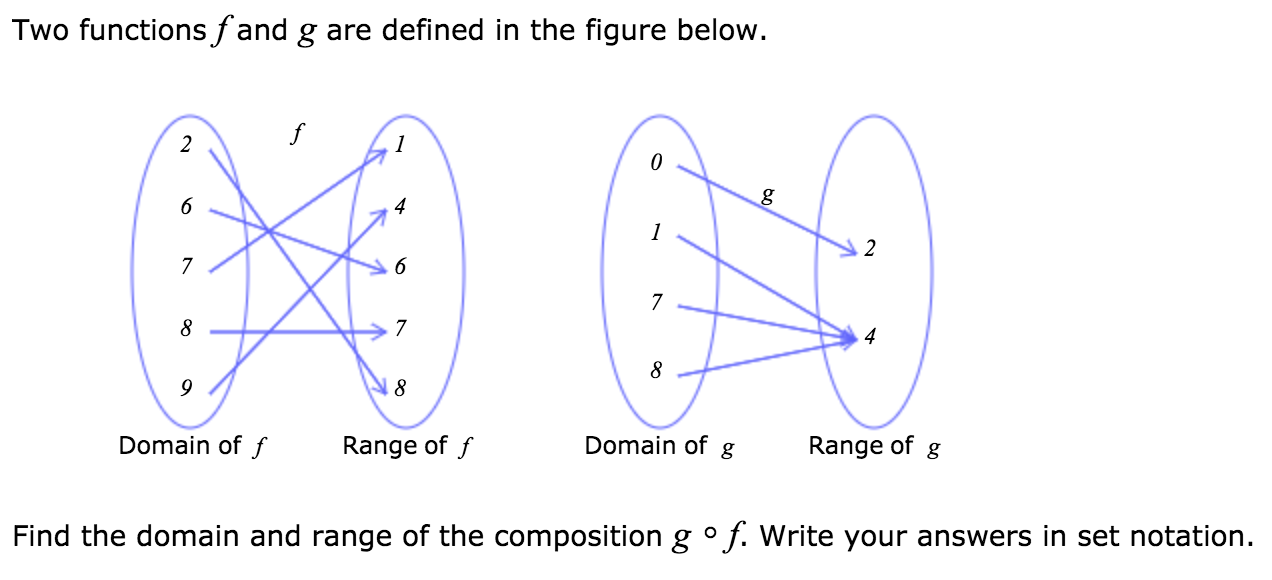
\includegraphics[scale=0.75]{Compositionwarmup}\begin{solution}
%		\textcolor{blue}{Domain: $\{2,7,8\}$ this is found by founding the domain of $f$ and then seeing which of these values are inputs for $g$.\\ Range: $\{4\}$ this is found by evaluating $g \circ f$ with the domain we found}
%	\end{solution}
%\end{enumerate}
%
%%%%%%%%%%%%%%%%%%%%%%% Day 18 Handouts %%%%%%%%%%%%%%%%%%%%%%
%
%\section*{Warm-Up}
%The volume $V(r)$ in cubic meters of a spherical balloon with a radius $r$ is given by the formula \[ V(r)=\frac{4}{3}\pi r^3\]
%\noindent
%The radius $W(t)$ in meters after $t$ seconds is given by \[W(t)=5t+3\]
%\noindent
%Write a formula, $M(t)$ for the volume of the balloon after $t$ seconds.
%\begin{solution}
%\textcolor{blue}{The formula asks for the volume of the balloon after $t$ seconds. We know that the volume of the balloon $V(r)=\frac{4}{3}\pi r^2$, and we know that the radius in terms of time is given by $W(t)=5t+3$. This means that $M(t)=(V\circ W)(t)=V(W(t))=\frac{4}{3}\pi (5t-3)^3$. }
%\end{solution}
%
%
%\section*{Practice Problems}
%Complete the following problems:
%\begin{enumerate}
%	\item For the following find the inverse of the function and evaluate $f^{-1}(2)$\\ \begin{center} \begin{tabular}{|l|l|l|l|l|}
%\hline
%$n$    & 3 & -4 & 1  & 2 \\ \hline
%$f(n)$ & 2 & 6  & -1 & 0 \\ \hline
%\end{tabular} \end{center} \vspace{1cm}
%\item Find the inverse of $f(x)=\frac{6x+2}{4x-5}$ \vspace{1cm}
%\item Let $f(x)$ be a one-to-one function. What point must be on the graph if $f(9)=11$?
%
%\end{enumerate}
%
%
%\section*{Concept Check}
%The average cost function of producing purple striped berets is given by the function $A=f(x)=3.5+\frac{2500}{x}$ where $x$ is the number of hats and $A$ is the average cost per hat when producing $x$ hats.\\ \vspace{1cm}
%
%\noindent
%Give the input, output, domain and range for this function.\\ \vspace{1.5cm}
%
%\noindent
%Find the inverse of this function.\\ \vspace{1.5cm}
%
%\noindent
%Evaluate $f^{-1}(16)$, and describe what this tells you about this problem.

%%%%%%%%%%%%%%%%%%%%%% Quadratic Functions %%%%%%%%%%%%%%%%%%%%%%

%\noindent
%A business has created a mathematical model based on market data for its profit, $P$ (in dollars), as function of the number of items sold, $x$. The model is given by the function \[ P(x)=-0.1x^2+150x-1400.\] How many units must be sold to maximize profit? What is the maximum profit?\\
%
%\subsection*{Things you need to know about Quadratic Functions}
%
%\noindent
%\textbf{General form: $f(x)=ax^2+bx+c$}\\
%
%
%\noindent
%\textbf{Vertex form: $f(x)=a(x-h)^2+k$}\\
%
%
%\noindent
%\textbf{Factored form: $f(x)=a(x-r_1)(x-r_2)$}\\
%
%\noindent
%\textbf{Example 1:}
%$f(x)=2x^2+5x+3$
%
%\noindent
%Describe the following features of the quadratic function. 
%\begin{itemize}
%	\item The shape
%	\item $y$-intercept
%	\item Write it in vertex form
%	\item Write it in factored form
%\end{itemize}
%
%\noindent
%\textbf{Example 2:}
%Find a formula for the parabola that goes through the points $(-5,0)$, $(3,0)$ and $(4,12)$\\
%
%
%\noindent
%\textbf{Example 3:}
%A concert venue holds a maximum of 1,000 people with ticket prices at \$30, the average attendance is 650 people. It is predicted that for every dollar the ticket price is lowered approximately 25 more people will attend. Create a function to represent the revenue generated from ticket sales and use this to find the maximum possible revenue.\\
%
%\noindent
%\textbf{Example 4:}
%Suppose a sunglass manufacturer determines the demand function for a certain line of sunglasses is given by $p=50-\frac{1}{4000}x$, where $p$ is the price per pair, and $x$ is the number of pairs sold. The fixed cost of producing this line of sunglasses is \$25,000 and each pair of sunglasses costs \$3 to produce. How many pairs of sunglasses should be produced and sold in order to maximize profits?\\
%
%\noindent
%\textbf{Warm-Ups:\\}
%
%\begin{problem}A tank is being filled with a liquid. The amount of liquid, $L$ in liters, after $t$ minutes is given by $L(t)=1.25t+73$. Answer the following questions:
%\begin{itemize}
%	\item Find $L^{-1}(x)$
%		\begin{solution}
%			\textcolor{blue}{\begin{align*}
%				y &= 1.25t+73\\
%				y-73 &= 1.25t+73-73\\
%				y-73 &= 1.25t\\
%				\frac{y-73}{1.25} &= \frac{1.25t}{1.25}\\
%				t&=\frac{y-73}{1.25}
%			\end{align*}
%			Thus $L^{-1}(y)=\frac{y-73}{1.25}$.}
%		\end{solution}
%	\item Find $L^{-1}(125)$
%		\begin{solution}
%			\textcolor{blue}{\begin{align*}
%				L^{-1}(125) &= \frac{125-73}{1.25}\\
%				&= \frac{52}{1.25}\\
%				&=41.6.
%			\end{align*}
%			Thus $L^{-1}(125)=41.6$.
%			}
%		\end{solution}
%	\item Interpret what the inverse tells us.
%		\begin{solution}
%			\textcolor{blue}{The inverse represents the amount of time in minutes it takes to fill the tank with a certain number of liters of liquid. }
%		\end{solution}
%\end{itemize}
%\end{problem}
%
%\begin{problem}
%Let $f(x)=\frac{1}{\sqrt{5x+1}}$ and $g(x)=-3x+2$. 
%\begin{itemize}
%	\item Find $(f \circ g)(x)$.
%		\begin{solution}
%			\textcolor{blue}{\begin{align*}
%				(f \circ g)(x) &= f(g(x))\\
%				&=\frac{1}{\sqrt{5(-3x+2))+1}}\\
%				&= \frac{1}{\sqrt{-15x+10+1}}\\
%				&=\frac{1}{\sqrt{-15x+11}}
%			\end{align*}}	
%		\end{solution}
%
%	\item Find $f^{-1}(x)$.
%		\begin{solution}
%			\textcolor{blue}{\begin{align*}
%				y &= \frac{1}{\sqrt{5x+1}}\\
%				y(\sqrt{5x+1}) &= 1\\
%				\sqrt{5x+1} &= \frac{1}{y}\\
%				5x+1 &= \frac{1}{y^2}\\
%				5x &= \frac{1}{y^2}-1\\
%				x&=\frac{1}{5y^2}-\frac{1}{5}.
%			\end{align*}
%			Thus $f^{-1}(y)=\frac{1}{5y^2}-\frac{1}{5}$.}
%		\end{solution}
%\end{itemize}
%\end{problem}
%
%\begin{problem}
%Factor completely:
%\begin{itemize}
%	\item $(x-11)^2+5(x-11)-24$
%		\begin{solution}
%			\textcolor{blue}{Let $u=(x-11)^2$. \begin{align*}
%				(x-11)^2+5(x-11)-24 &= u^2+5u-24\\
%				&=(u+8)(u-3)\\
%				&=(x-11+8)(x-11-3)\\
%				&=(x-3)(x-14)
%			\end{align*}}
%		\end{solution}
%	\item $3(8x+3)^2(7x-6)-(8x+3)(7x-6)^2$
%		\begin{solution}
%			\textcolor{blue}{The greatest common factor between the two is $(8x+2)(7x-6)$. \begin{align*}
%				3(8x+3)^2(7x-6)-(8x+3)(7x-6)^2 &= (8x+3)(7x-6)(3(8x+3)-(7x-6))\\
%				&=(8x+3)(7x-6)(24x9-7x+6)\\
%				&= (8x+3)(7x-6)(17x+15)
%			\end{align*}}	
%		\end{solution}
%
%\end{itemize}
%
%\end{problem}
%
%\noindent
%\textbf{Concept Check:}
%\begin{problem}
%Consider the following function: 
%\[ f(x)=\sqrt{4-x}+7 \]
%
%\noindent
%The domain of the function is $(-\infty, 4]$ and the range is $(-\infty, \infty)$. 
%
%\begin{enumerate}
%	\item Find $f^{-1}(x)$.
%		\begin{solution}
%			\textcolor{blue}{\begin{align*}
%				y&=\sqrt{4-x}+7\\
%				y-7 &= \sqrt{4-x}\\
%				(y-7)^2 &= 4-x\\
%				(y-7)^2 -4 &= -x\\
%				-(y-7)^2+4 &=x
%			\end{align*}
%			Thus $f^{-1}(y)=-(y-7)^2+4$.}
%		\end{solution}
%	\item What is the domain of $f^{-1}(x)$?
%		\begin{solution}
%			\textcolor{blue}{The rule tells us that we switch the domain and range from the original function. This implies that the domain of $f^{-1}$ is the range of $f(x)$. Thus the domain for $f^{-1}$ is $(-\infty, \infty)$.}
%		\end{solution}
%	\item What is the range of $f^{-1}(x)$?
%		\begin{solution}
%			\textcolor{blue}{The rule tells us that we switch the domain and range from the original function. This implies that the range of $f^{-1}$ is the domain of $f(x).$ Thus the range of $f^{-1}$ is $(-\infty, 4]$.} 
%		\end{solution}
%\end{enumerate}
%\end{problem}
%
%\begin{problem}
%\begin{itemize}
%	\item Find an equation for the parabola that passes through the points $(-1,0)$, $(3,0)$ and $(5,10)$.
%		\begin{solution}
%			\textcolor{blue}{Since we were given the $x$-intercepts of the equation, we will use intercept form, $y=a(x-r_1)(x-r_2)$. This gives us $y=a(x+1)(x-3)$ so we need to solve for $a$. We do this by using the point we haven't used yet. \begin{align*}
%				10 &= a(5+1)(5-3)\\
%				10 &= a(6)(2)\\
%				\frac{10}{12} &= a\\
%			\end{align*}
%			Thus $a=\frac{5}{6}$ and our equation is $y= \frac{5}{6}(x+1)(x-3)$.}
%		\end{solution}
%	\item Find an equation for the parabola that has a vertex of $(4,5)$ and passes through the point $(0,-6)$.
%		\begin{solution}
%			\textcolor{blue}{Since we were given the vertex and a point, we will use vertex form, $y=a(x-h)^2+k$, where $(h,k)$ is the vertex. This give us $y=a(x-4)^2+5$ so we need to solve for $a$. We do this by using the point we haven't used yet. \begin{align*}
%				-6 &= a(0-4)^2+5\\
%				-6 &= a(-4)^2+5\\
%				-11 &= a(-4)^2\\
%				-11 &= 16a\\
%				\frac{-11}{16} &= a
%			\end{align*}
%			Thus $a=\frac{-11}{16}$ and our equation is $y=\frac{-11}{16}(x-4)^2+5$}
%		\end{solution}
%\end{itemize}	
%\end{problem}
%
%
%\begin{problem}
%The braking distance $D(v)$ (in meters) of a certain car moving at a certain velocity $v$ is given by $D(v)=\frac{v^2}{22}$. The car's velocity $B(t)$ (in meters per second) $t$ seconds after starting is given by $9t$. How many meters will it take the car to stop if it has been driving for 30 seconds? 
%\end{problem}
%
%
%
%\begin{problem}
%Scientists are studying the temperature on a distant planet. They find that the temperature $T$ depends on the height $h$ (in kilometers) above the planet's surface. The relationship is as follows: \[T(h)=48.5-2.5h.\] Use this to answer the following questions: 
%\begin{enumerate}
%	\item In practical terms describe $T^{-1}(h)$.
%	\item Find $T^{-1}(h)$.
%	\item What is $T^{-1}(33)$?
%\end{enumerate}	
%\end{problem}
%
%
%
%\begin{problem}
%A ball is thrown from an initial height of 2 meters with an initial upward velocity of 30 meters per second. The ball's height $h$ (in meters) is given by \[h(t)=2+30t-5t^2.\] Use this to answer the following:
%\begin{enumerate}
%	\item Find all values for which the ball is at 12 meters.
%	\item When does the ball touch the ground?
%	\item What is the maximum height the ball reaches and when does it reach that height?
%\end{enumerate}
%\end{problem}
%
%
%\begin{problem}
%	Write the equation for the quadratic function that contains the following points $(-1,0)$, $(3,0)$ and $(5,4)$.
%\end{problem}
%
%
%\begin{problem}
%	Write the equation for the quadratic function that contains has a vertex at $(3,4)$ and passes through the point $(8,-4)$.
%\end{problem}
%
%
%\begin{problem}
%	The length of a rectangle is 8 yards less than 3 times it's width. The area of the rectangle is 35 square yards. Find the dimensions of the rectangle.
%\end{problem}
%
%
%\begin{problem}
%	Answer the following questions about the following quadratic equation \[x^2-6x+11\]
%	\begin{enumerate}
%		\item Is the vertex a maximum or minimum?
%		\item Where does the vertex occur?
%	\end{enumerate}
%\end{problem}
%
%
%\begin{problem}
%Find the zeros of the following quadratic equation \[-3x^2+6x+1\]	
%\end{problem}
%
%
%\begin{problem}
%When an apple orchard owner plants 65 trees on an acre of ground, he gets an average yield of 1500 apples per tree. For each additional tree planted per acre, the annual yield per tree drops by 20 apples. Let $x$ represent the number of additional trees above 65.
%\begin{enumerate}
%	\item Determine an equation that represents the yield of apples the orchard owner will get per year.
%	\item How many trees should the owner plant in order to maximize the output of the orchard?
%	\item What is the maximum amount of apples will the orchard produce?
%\end{enumerate}
%\end{problem}
%
%
%\begin{problem}
%	A charter flight charges a fee of \$300 per person plus \$2 per person for each unsold seat on the plane. The plane holds 200 passengers. 
%	\begin{enumerate}
%		\item Determine an equation that represents the revenue based on number of passengers $x$
%		\item How many passengers should ride on the plane to maximize revenue?
%		\item What is the maximum revenue the company can make?
%	\end{enumerate}
%\end{problem}


%\begin{enumerate}
%	\item Determine an equation for the rational function that has:
%		\begin{itemize}
%			\item $f(x)$ has a zero at $x=2$
%			\item $f(x)$ has a vertical asymptote at $x=-1$
%			\item $f(x)$ has a horizontal asymptote at $y=3$
%		\end{itemize} 
%	\item A patient is being treated for a chronic illness. The concentration $C(x)$ in $g$ per $mL$ of a certain medication in the patient's bloodstream $x$ weeks after taking the medication is approximated by $C(x)=\frac{8x^2-31x+35}{4x^2-16x+17}$. During what week is the largest concentration in the patient's bloodstream? How much is in their bloodstream during that week? As time passes how much medication will be in the patient's bloodstream? 
%	\item Answer the following questions about the rational function $f(x)=\frac{x^2+3x-18}{x^2-4}$. Identify the: 
%		\begin{itemize}
%			\item Domain
%			\item Vertical Asymptote
%			\item Horizontal Asymptote
%			\item Zeros
%			\item $y-$intercept
%		\end{itemize} 
%	\item The cost $C$ in millions of dollars of removing $x\%$ of pollutant from a lake is given by $f(x)=\frac{50x}{100-x}$, where $0 \leq x \leq 100$. Use this information to answer these questions:
%		\begin{itemize}
%			\item Evaluate $f(60)$ and interpret what it means in context of the problem
%			\item If a company has 25 million dollars to spend how much pollutant can they remove?
%			\item What amount of money does a company need to have in order to remove 95\% of the pollution?
%			\item A current law states that in order for a state to receive federal funding at least 10\% of the funding must be utilized clean water ways. If the government is funding 900 million to a certain state how much pollutant can they remove from the lake?
%		\end{itemize} 
%	\item The number of random facts a person can learn depends on the number of minutes, $m$, they spend studying. This is represented by the following graph. Use the graph to find an equation that represents the number of facts a person can learn. 
%		\begin{center}
%			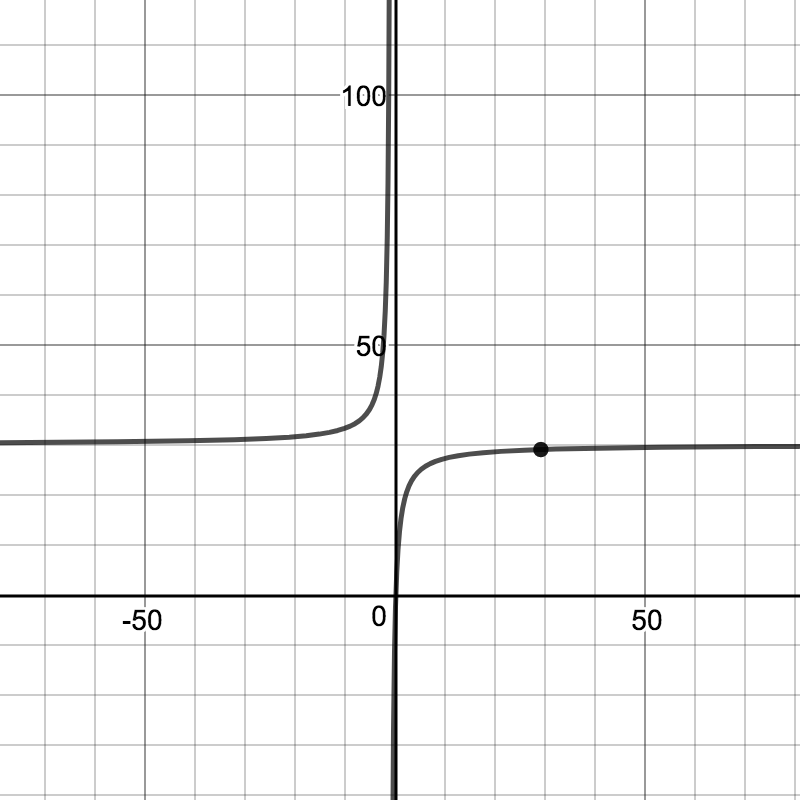
\includegraphics[scale=0.25]{rationalfunction3}
%		\end{center} 
%\end{enumerate}


%\subsection*{Problem Set 2}
%\begin{enumerate}
%\item A company that produces telephones has determined that the monthly fixed cost is \$12,000 and it costs \$30 to manufacture each telephone. Use this information to answer the following questions.
%	\begin{itemize}
%		\item Write a function that represents the average cost per telephone.
%		\item Determine an appropriate domain for the function.
%		\item As the number of telephones the company produces increases, what does the average cost become?\\[4mm]
%	\end{itemize}
%
%	
%	
%\item A scientist is studying the temperature in a certain region of a remote planet. She approximates the temperature, $T$ in degrees Celsius in that region $x$ years after the planet's origin to be the following \[T=\frac{3x^2-13x+8}{x^2-4x+8}.\] In what year was the temperature the coolest? What was the coolest temperature? Does the temperature of the planet ever level off? If so, what does the temperature tend to?
%\end{enumerate}

%\section*{Polynomial Functions}
%\subsection*{Things to know about Polynomial Functions}
%\begin{itemize}
%	\item How does the degree of a polynomial function affect the ends of the graph?
%	\item How does the leading coefficient affect the ends of the graph?
%	\item What generalization can you make about the ends of the graph based on the degree of the polynomial and the leading coefficient?
%	\item How does the degree of the polynomial relate to the number of zeros it has?
%	\item How does the degree of the polynomial relate to the number of turns a graph has?
%\end{itemize}
%
%\subsection*{Examples}
%\begin{enumerate}
%	\item Determine the degree, leading coefficient, and zeros of the following polynomial equations. Sketch a rough graph by hand and check your answers on your graphing calculator. \begin{enumerate}
%	\item $y=x^3-x^2-6x$
%	\item $y=-\frac{1}{2}(x+3)(x-2)(x+1)(x-5)$
%	\item $y=-x^4+13x^2-36$
%	\end{enumerate}
%	\item Determine a possible equation for the following graphs. Verify your answers on your graphing calculator. \begin{enumerate}
%	\item 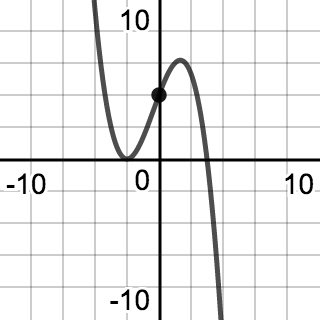
\includegraphics[scale=0.25]{cubicpractice.png}
%	\item 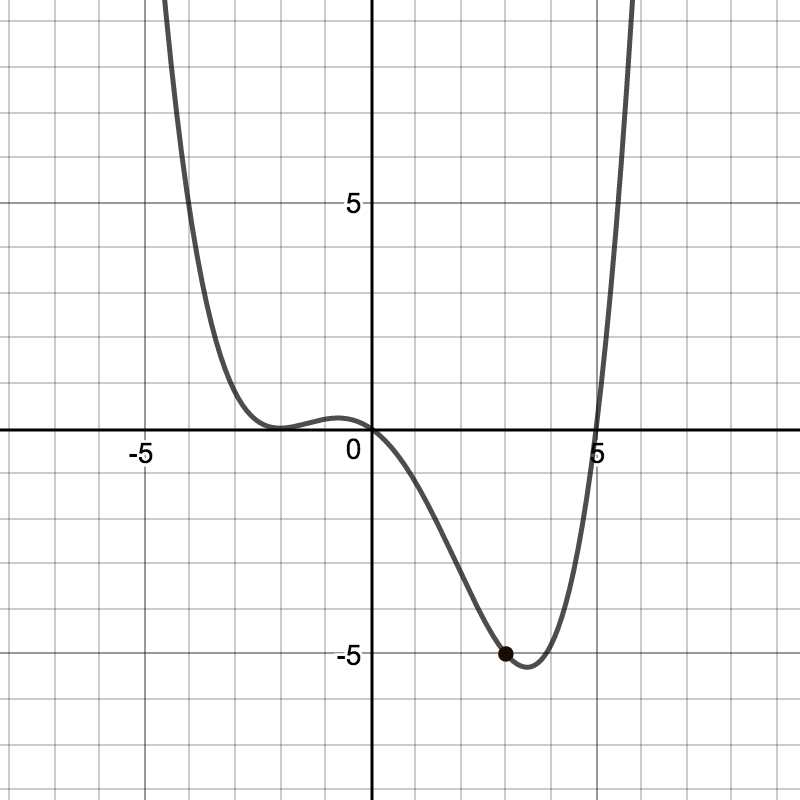
\includegraphics[scale=0.15]{quarticpractice.png}
%	\end{enumerate}
%	\item Based on actuarial life tables, the average number of years of life remaining for a female of age $x$ (up to 100) can be approximated by the function \[N(x)=0.0000004x^4-0.00004x^3+0.002x^2-1.0191x+81.955.\] Use this to answer the following questions: \begin{enumerate}
%	\item Graph this function in an appropriate window.
%	\item What does this graph tell us in practical terms?
%	\item What is the $y$-intercept? What does it mean in practical terms?
%	\item What is the degree of this function?
%	\item What is the leading coefficient of this function?
%	\item Is this function increasing or decreasing on the implied domain? What does this tell us in practical terms?
%	\item Why does it make sense that life expectancy increases as the age of the female increases?
%	\end{enumerate}	
%	\item A $12 \times 8$ rectangular piece of cardboard is folded into an open top box. This is possible by cutting squares from each of the corners. \begin{enumerate}
%	\item Determine a formula for the volume of the box.
%	\item Find the maximum possible volume.
%	\end{enumerate}	
%	\item For a particular pair of sunglasses, it is determined that the cost function is given by \[C(x)=0.00003x^3+7x+1,500\] and the revenue function is given by \[R(x)=-0.01x^2+40x\] where $x$ is the number of sunglasses produced and sold. Find a function to represent the profit as a function of $x$. Determine the number of units that should be sold in order to maximize profit. What is the maximum profit? 
%\end{enumerate}

%\section*{Rational Functions}
%\subsection*{Introductory Example}
%A clothes dryer is purchased for \$750, and electricity to run it costs approximately \$95 per year. Write a function that represents the average cost per year of operating the dryer. Graph this function in an appropriate window.\\[2mm]
%
%\subsection*{Things to know about Rational Functions}
%General form:\\[2mm]
%Domain of a rational function: \\[2mm]
%Zeros of a rational function:\\[2mm]
%Vertical Asymptotes: \\[2mm]
%Horizontal Asymptotes: 
%\subsection*{Example to Practice with}
%\[f(x)=\frac{3x-2}{x-1}\]
%
%\subsection*{Examples}
%For the following function identify the domain and write equations for all the asymptotes. Verify your answer by graphing.
%\[f(x)=\frac{2x+1}{x^2-16}\]
%
%Find an equation for the following rational equations.\\
%\begin{center}
%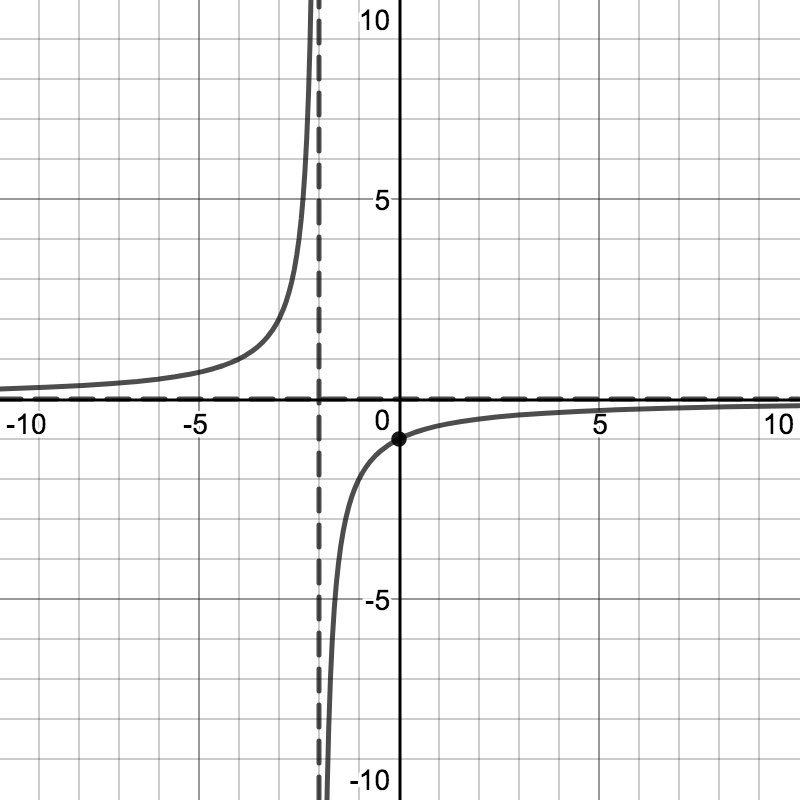
\includegraphics[scale=0.15]{graph2.png}\\[10mm]
%\end{center}
%
%\begin{center}
%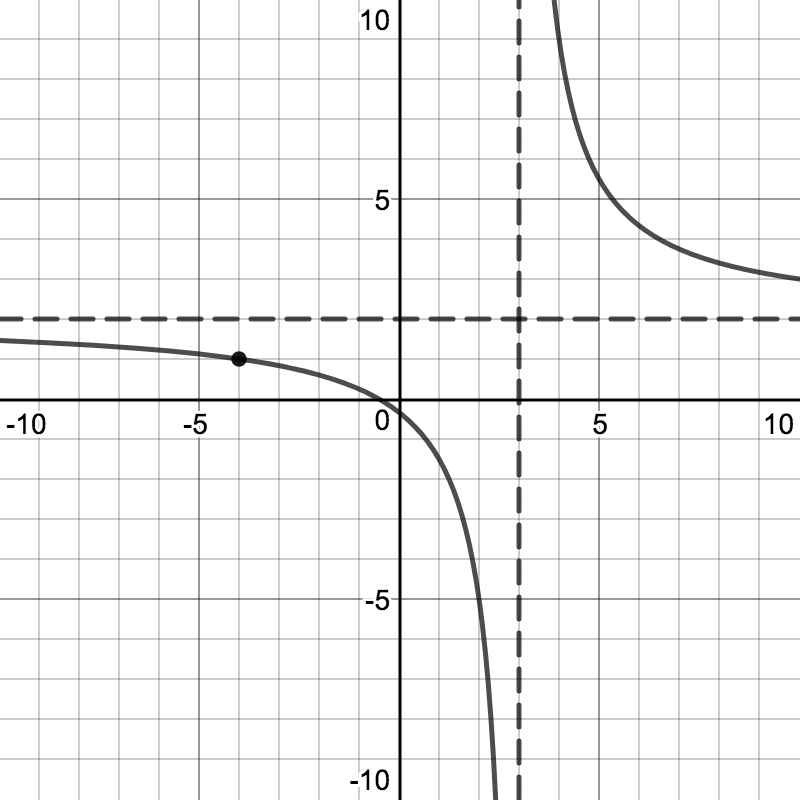
\includegraphics[scale=0.15]{graph1.png}
%\end{center}
%
%\noindent
%A company that assembles bicycles has determined that a new employee can assemble $M(d)$ bicycles per day after $d$ days of on-the-job training, where $M(d)=\frac{100d^2}{3d^2+10}$. After how many days of training would an employee be able to assemble 25 bicycles per day?\\[4mm]
%
%
%\subsection*{Problem Set 1}
%\begin{enumerate}
%	\item Determine an equation for the rational function that has:
%		\begin{itemize}
%			\item $f(x)$ has a zero at $x=2$
%			\item $f(x)$ has a vertical asymptote at $x=-1$
%			\item $f(x)$ has a horizontal asymptote at $y=3$
%		\end{itemize}
%	\item A patient is being treated for a chronic illness. The concentration $C(x)$ in $g$ per $mL$ of a certain medication in the patient's bloodstream $x$ weeks after taking the medication is approximated by $C(x)=\frac{8x^2-31x+35}{4x^2-16x+17}$. During what week is the largest concentration in the patient's bloodstream? How much is in their bloodstream during that week? As time passes how much medication will be in the patient's bloodstream?
%	\item Answer the following questions about the rational function $f(x)=\frac{x^2+3x-18}{x^2-4}$. Identify the: 
%		\begin{itemize}
%			\item Domain
%			\item Vertical Asymptote
%			\item Horizontal Asymptote
%			\item Zeros
%			\item $y-$intercept
%		\end{itemize}
%	\item The cost $C$ in millions of dollars of removing $x\%$ of pollutant from a lake is given by $f(x)=\frac{50x}{100-x}$, where $0 \leq x \leq 100$. Use this information to answer these questions:
%		\begin{itemize}
%			\item Evaluate $f(60)$ and interpret what it means in context of the problem
%			\item If a company has 25 million dollars to spend how much pollutant can they remove?
%			\item What amount of money does a company need to have in order to remove 95\% of the pollution?
%			\item A current law states that in order for a state to receive federal funding at least 10\% of the funding must be utilized clean water ways. If the government is funding 900 million to a certain state how much pollutant can they remove from the lake?
%		\end{itemize}
%	\item The number of random facts a person can learn depends on the number of minutes, $m$, they spend studying. This is represented by the following graph. Use the graph to find an equation that represents the number of facts a person can learn. 
%		\begin{center}
%			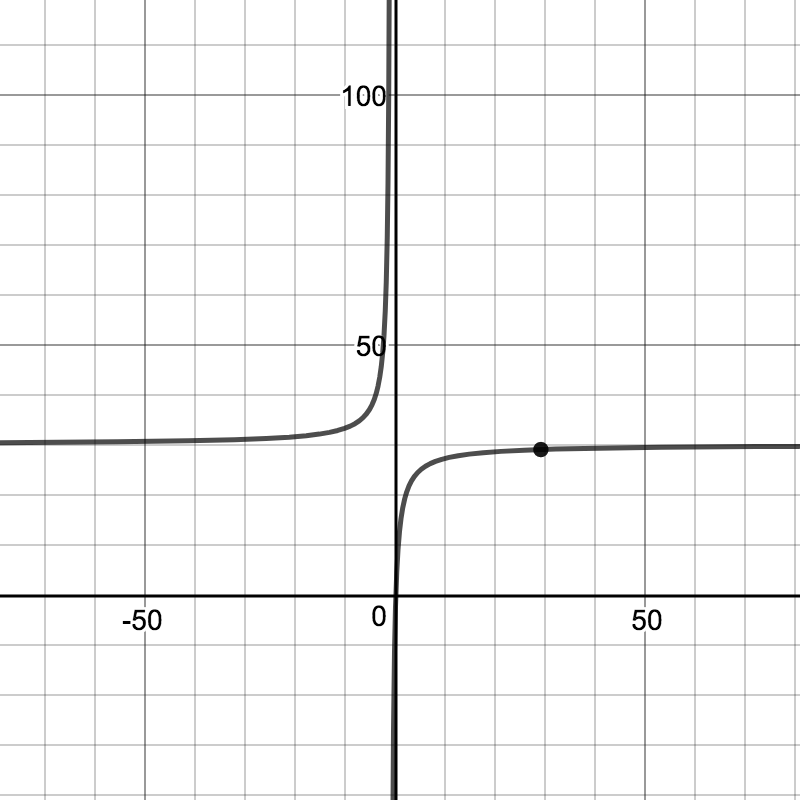
\includegraphics[scale=0.25]{rationalfunction3}
%		\end{center}
%\end{enumerate}
%
%
%\subsection*{Problem Set 2}
%\begin{enumerate}
%\item A company that produces telephones has determined that the monthly fixed cost is \$12,000 and it costs \$30 to manufacture each telephone. Use this information to answer the following questions.
%	\begin{itemize}
%		\item Write a function that represents the average cost per telephone.
%		\item Determine an appropriate domain for the function.
%		\item As the number of telephones the company produces increases, what does the average cost become?\\[4mm]
%	\end{itemize}
%	
%\item A scientist is studying the temperature in a certain region of a remote planet. She approximates the temperature, $T$ in degrees Celsius in that region $x$ years after the planet's origin to be the following $T=\frac{3x^2-13x+8}{x^2-4x+8}$. In what year was the temperature the coolest? What was the coolest temperature? Does the temperature of the planet ever level off? If so, what does the temperature tend to?
%
%\end{enumerate}


%\noindent
%Let's talk about rabbits $\cdots$\\[4mm]
%\begin{center}
%\begin{tabular}{c|c}
%Time & Number of Rabbits \\ \hline
%0    & 2                 \\
%1    & 6                 \\
%2    & 18                \\
%3    & 54                \\
%4    & 162               \\
%5    & 486              
%\end{tabular} \\[5mm]
%\end{center}
%
%
%\noindent
%Nathan has \$100 to open a savings account. He found an account that offers 2.5\% interest compounded annually. Write a function to represent the balance in the account as a function of time in years, assuming the initial deposit and all subsequent interest is kept in the account. Graph this function in an appropriate window.
%
%
%\noindent
%\subsection*{Things to know about Exponential functions}
%What is the general form of on exponential function? \\
%What differentiates an exponential function from the other types of functions we have studied? \\
%What is the domain of an exponential function? The range? The intercept(s)? The asymptote(s)? \\
%What determines whether an exponential function is increasing or decreasing?\\
%What is the formula for compound interest if it is compounded annually? $n$ times per year? continuously? 
%
%\subsection*{Examples}
%\noindent
%Determine the for $y=C \cdot b^x$ that passes through the points $(1,12)$ and $(3,192)$.\\[5mm]
%
%\noindent
%A person plans to invest \$5,000 into a money market account. Find the interest rate required for the money to grow to \$45,000 in 30 years if the interest is compounded quarterly.\\[5mm]
%
%\noindent
%Bacteria from raw eggs has come into contact with the onions and celery you are going to put into your potato salad. Initially there were 500 bacteria present; one hour later there were 4,000 bacteria present in the salad. The population of the bacteria in the salad can be modeled by a exponential function $y=C \cdot b^t$, where $t$ is measured in hours. Create a function that represents this situation, and use the graph to determine the number of hours it takes for the bacteria's population to double in size. \\[5mm]
%
%
%\noindent
%\$100 is invested into an account bearing 12\% interest. What will the balance in the account be in 10 years if $\ldots$\\
%interest is compounded annually?\\
%interest is compounded quarterly?\\
%interest is compounded monthly?\\
%interest is compounded daily?\\[5mm]
%
%\noindent
%A radioactive substance has a half-life of 20 days. If the initial amount is 25 grams, write a function to represent the amount of substance remaining after $t$ days.\\[5mm]
%
%\begin{problem}
%	A population of 800 beetles is growing each month at a rate of 8\%. Write a function that represents the number of beetles at time $x$. About how many beetles will there be in 2 years?
%\end{problem}
%
%\begin{problem}
%	The half-life of ibuprofen is given by the formula \[ R=M(0.5)^t \] where $t$ is the time in hours and the dosages are measured in milligrams. If a person took a 200 milligram dose 2 hours ago, how much is currently left in their blood stream? A person has 30 milligrams in their body 1 hour after taking the medication, how much was their original dosage? 
%\end{problem}
%
%\begin{problem}
%	You recently bought a new computer for \$1,500 and were astounded when you did research that people with the same model computer who bought it 2 years before can only sell their machines for \$800. Write an equation to represent depreciation of your computer. When will the computer be valued at \$200?
%\end{problem}
%
%\begin{problem}
%	The half-life of caffeine is 5 hours. A grande French roast has 330 milligrams of caffeine. Using this information write an equation to represent the amount of caffeine in your bloodstream after $t$ hours in the form $y=Pe^{rt}$. At what time will the caffeine in your body no longer be effective (for most adults this occurs when there are about 20 milligrams or less in your bloodstream)?
%\end{problem}
%
%\begin{problem}
%	A certain termite colony triples in size every 2 weeks. The pest control came to your house a month ago and counted that you had 500 termites in your house. Write a function that represents the number of termites in your house in terms of $t$ where $t$ represents the number of weeks since the initial inspection. Since that inspection it has been 6 weeks and they termite people have come back to spray termite spray. How many termites are they exterminators going to exterminate?
%\end{problem}
%
%\subsection*{Warm-up Questions}
%\begin{problem}
%	Graph the following rational function:
%	\[f(x)=\frac{-12}{x^2+8x+12}\]
%	
%	\begin{solution}
%		\textcolor{blue}{Here is the graph that you should have seen. This was created using Desmos.}\\
%		\begin{center}
%		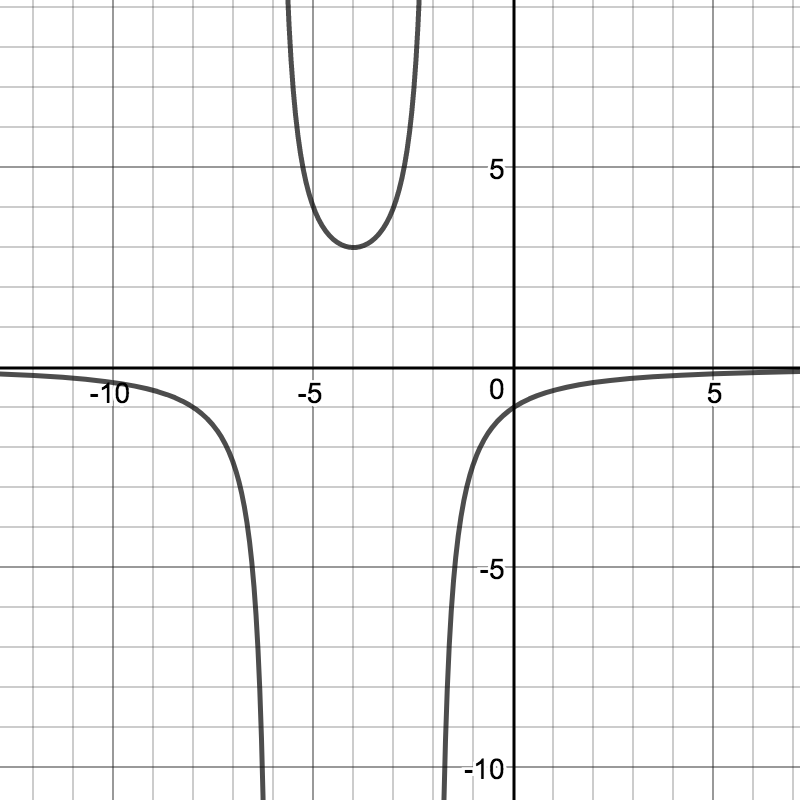
\includegraphics[scale=0.5]{rationalsolution}
%		\end{center}
%	\end{solution}
%	
%	Identify the:
%	\begin{itemize}
%		\item Horizontal Asymptote: 
%			\begin{solution}
%				\textcolor{blue}{Since the degree in the denominator is bigger than the degree in the numerator, the horizontal asymptote is $y=0$.This can also be seen in the graph above.}
%			\end{solution}
%		\item Vertical Asymptote(s):
%			\begin{solution}
%				\textcolor{blue}{To find the vertical asymptotes, we set the denominator equal to zero and solve for $x$. That is
%				\begin{align*}
%					0 &= x^2+8x+12\\
%					&=(x+2)(x+6)\\
%				\end{align*}
%				This implies that there are vertical asymptotes at $x=-6$ and $x=-2$. This can also be seen in the graph of the function above.}
%			\end{solution}
%		\item Zeros of the function
%			\begin{solution}
%				\textcolor{blue}{To find the zeros we set the numerator equal to $0$ and solve. That is we have $0=-12$. This does not make sense which implies this function has no zeros.}
%			\end{solution}
%		\item $y$-intercept
%			\begin{solution}
%				\textcolor{blue}{The $y$-intercept occurs when we plug in 0 for $x$ and simplify. We see that
%				\begin{align*}
%					f(0) &= \frac{-12}{0^2+8(0)+12}\\
%					&=\frac{-12}{0+0+12}\\
%					&=\frac{-12}{12}\\
%					&=-1
%				\end{align*}
%				Thus the $y$-intercept is $(0,-1)$.}
%			\end{solution}
%	\end{itemize}
%\end{problem}

%
%\begin{problem}
%	A city's population has been growing exponentially over the past several years. In 2005, the population was 420,000 people and in 2016 the population was 630,000 people. 
%	\begin{itemize}
%		\item Write an equation that represents the population where $t$ is time in years since 2000.
%		\item What was the population estimated to be in 2010?
%		\item When will the population be 1,000,000 people?\\[9cm]
%	\end{itemize}
%\end{problem}
%
%\begin{problem}
%	Tricia drinks coffee every morning before work. The brand of coffee Tricia purchases indicates that it has 190 milligrams per serving. One day Tricia had some lab work completed and they found that Tricia had 80 milligrams of caffeine in her body approximately 6 hours after she had finished her morning coffee. Find the half life of the caffeine in Tricia's body.
%\end{problem}
%
%\newpage
%
%\begin{problem}
%	An outbreak of E. Coli occurred during January of this year due to people eating romaine lettuce. Jorge purchased romaine lettuce in January from a contaminated source. When Jorge bought his lettuce there were 25 E. Coli bacteria present. At the time Jorge ingested his lettuce, 2 days after he purchased it, there were 60 E. Coli bacteria present. The amount of bacteria a human needs to have present in order to get sick with this specific type of bacteria is 100. Assuming Jorge's system doesn't fight off the infection and the bacteria keep growing at the same rate, when will Jorge get sick? \\[9cm]
%\end{problem}
%
%\begin{problem}
%	The sounds humans can hear is measured using decibels. The formula to find the number of decibels a sound is given by \[ d=10\log \left(\frac{P}{P_0}\right)\] where $P$ is the power of the intensity of the sound and $P_0$ is the weakest sound a human ear can hear.\\
%	
%	\noindent
%	A hot water pump  has a noise rating of 50 decibels while a certain dishwasher has a noise rating of 62 decibels. How much more intense is the dishwasher noise than the hot water pump noise? (Hint: solve for the power of intensity of each and compare the two values)
%\end{problem}
%
%\newpage
%
%\begin{problem}
%	In 2010 the world had a population of 6.9 billion people. Last year the world population was recorded at 7.6 billion people. Use this information to answer the following questions.
%	\begin{itemize}
%		\item Write an equation that represents the world population.
%		\item By the end of this year, what is the population expected to be?
%		\item Ecologists estimate that the carrying capacity of the Earth is 10 billion people. During what year does our model estimate the carrying capacity to be reached? \\[9cm]
%	\end{itemize}	
%\end{problem}
%
%\begin{problem}
%	In 1935 Charles Richter defined the magnitude of an earthquake to be \[M=\log \left( \frac{I}{S} \right) \] where $I$ is the intensity of the earthquake (measured by a seismograph) and $S$ is the standard intensity of an earthquake.\\
%	
%	\noindent
%	On January 12, 2010 had an earthquake of magnitude 7.0. Yesterday morning at 6 a.m. a 3.0 magnitude earthquake occurred in Fontana, California 439 miles from Tucson. How many times strong was the earthquake in Haiti than the earthquake in California yesterday?
%\end{problem}
%
%\newpage
%
%\begin{problem}
%	Carbon-14 is a radioactive isotope that is used to help date the ages of bones that are found in archeological digs. It has a half-life of 5370 years. Use this information to answer the following questions:
%	\begin{itemize}
%		\item Create an equation to represent the amount of Carbon-14 left in a bone after $t$ years.
%		\item How long would it take for a bone to have 60\% of the original Carbon-14 left in it?
%		\item A recent found fossil is estimated to have been around ~39,000 years ago. How much Carbon-14 should the scientists expect it to contain? \\[9cm]
%	\end{itemize}
%\end{problem}
%
%\begin{problem}
%	Consider the following logarithmic function with base $b>1$ \[y=\log_b(Ax+B)+C\] where $A, B$, and $C$ are positive constants.
%	\begin{itemize}
%		\item Determine the exact values of all intercepts and asymptotes.
%		\item Sketch an accurate graph of $y=\log_b(Ax+B)+C$.
%	\end{itemize}
%\end{problem}


%\section*{Logarithms}
%\$1 is invested in an account earning 5\% interest compounded annually. How long will it take the amount in the account to grow to \$2.\\
%
%\noindent
%Consider $y=2^x$:
% 
%\subsection*{Things to know about logarithmic functions}
%\begin{enumerate}
% 	\item What is a logarithm?
% 	\item What is the notation for logarithm? What is the exponential equivalent of a logarithm? 
% 	\item How do you evaluate simple logarithmic expressions?  
% 	\item What is the common logarithmic function? The natural logarithmic function? 
% 	\item What is the domain/range/intercept/asymptote of a logarithmic function? 
%\end{enumerate}
%
%
%\noindent
%Find the domain and intercepts of the logarithmic function, and sketch the graph $f(x)=\log(3x-2)$.\\
%
%\noindent
%The amount of radioactive material in a 200-gram sample of bismuth can be modeled by the function $A(t)=200e^{-0.1386t}$, where $t$ is time in days. What is the half-life of this radioactive material?\\
%
%\noindent
%A population of 1000 bacteria is on the kitchen counter. The amount of time, in hours, that it takes the population to reach $x$ bacteria is given by $f(x)=16 \cdot \ln\left( \frac{x}{1000}\right)$. How many bacteria will their be in 3 hours. \\
%
%\subsection*{Concept Check}
%The half-life of caffeine is 5 hours. Pepsi Zero Sugar has 115 milligrams of caffeine. Using this information write an equation to represent the amount of caffeine in your bloodstream $t$ hours after drinking Pepsi Zero Sugar.

%\section*{Properties of Logarithms}
%\subsection*{Things to know about the Properties of Logarithms}
%What is the property for a logarithm of an input that is multiplied? \\
%What is the property for a logarithm of an input that is divided? \\
%What is the property for a logarithm of a power?\\
%What is the inverse property of logs/exponential functions?\\
%
%\noindent
%Use the properties of logs to rewrite the following as a single logarithmic expression:\\
%
%\noindent
%$\ln(6x)+\frac{1}{2}\ln(x)-\ln(2x)$\\
%
%\noindent
%$\log(5z)-\log(x)-3\log(3y)+\log(t)$\\
%
%\noindent
%$2\log_2(x^2)+\log_2(y)-4\log_2(P)-\frac{1}{3}\log_2(Q)+\log_2(z)$\\
%
%
%
%\noindent
%Use the properties of logarithms to expand each expression as much as possible:\\
%
%\noindent
%$\ln(10xe^3x)$\\
%
%\noindent
%$\log\left(\frac{2x^4}{y\sqrt{z}} \right)$\\
%
%\noindent
%$\log_5(\sqrt{5z})$\\
%
%
%\noindent
%Use the natural logarithm and a property of logarithms to solve: $4(3)^x=20$.\\
%
%
%\noindent
%Use property of logarithms to solve:\\
%
%\noindent
%$\log(-x-2)+\log(1-x)=1$\\
%
%\noindent
%$\log_3(3x+17)-\log_3(x+1)=2$	

\section*{Applications of Exponential and Logarithmic Functions}
\begin{problem}
	A cup of coffee that is initially $125^\circ$F is placed in a room kept at a constant $72^\circ$F. The temperature of the coffee, $T$ as a function of time is given by $T(x)=72+53(0.8)^x$, where $x$ is measured in minutes. How long will it take the coffee to cool to $100^\circ$F?
\end{problem}



\begin{problem}
	A radioactive isotope of bismuth has a half-life of $5$ days. After how many days will 20\% of the isotope remain?
\end{problem}



\begin{problem}
	The world population has been growing roughly exponentially for the past 30 years. In 1987, the world population was approximately 5 billion. In 1998, the world population was approximately 6 billion. Find an exponential equation of the form $y=Ce^{kt}$ which models the population with $t$ representing the number of years 1987. Use at least 6 decimal places for the value of $k$. What does the model predict the population was in 2000?
\end{problem}



\begin{problem}
	Suppose Matt wants to have \$10,000 saved in 9 years. How much should he invest today at 3.4\% compounded continuously in order to reach his goal?
\end{problem}



\begin{problem}
	A radioactive isotope of bismuth has a half-life of 5 days. After how many days will a 200-gram sample decay to 20 grams of radioactive material?
\end{problem}



\begin{problem}
	The doubling time for an investment is given by the equation $T=\frac{\ln(2)}{\ln(1+r)}$ where $r$ is the interest rate in decimal form. At what interest rate would you need to invest in order to double your investment in 10 years?
\end{problem}



\begin{problem}
	Suppose after 2500 years an initial amount of 1000 grams of radioactive substance has decayed to 75 grams. What is the half-life of the substance?
\end{problem}



\begin{problem}
	The concentration of a pollutant in the atmosphere increases according to the exponential growth model $A=Pe^{rt}$, where time is measured in years and $r=0.0035$. In 1990, the concentration was 56 parts per million. Clean-up procedures will be initiated when the concentration reaches 70 parts per million. According to the model, in what year will that occur?
\end{problem}



\begin{problem}
	Air pressure, $P$, decreases exponentially with the height above the surface of the earth. At the top of Mount Everest, height 8848 meters, the air pressure is about 34.6\% of the air pressure at sea level. Approximate the air pressure as a percentage of the sea level value at the top of Mount Kilimanjaro, height 5895 meters.
\end{problem}



\begin{problem}
	What is the doubling time for a population of rabbits that grows from 120 to 500 in 12 months?
\end{problem}

\begin{problem}
	A pork roast is removed from the freezer ($25^\circ$F) and placed in a room ($75^\circ$F). The number of minutes it takes the temperature of the roast to reach $x$ degrees F is given by the formula $T=f(x)=\frac{100}{3}\ln\left(\frac{50}{75-x}\right)$. Find and interpret $f^{-1}(70)$.
\end{problem}

\begin{problem}
	New employees are given an initial exam and then retested monthly with an equivalent exam. The average scores for the employees can be expressed as $S(t)=76-6\cdot \log_{3}(t+1)$ where $t$ is measured in months since the initial exam. After approximately how many months would the average score be 54?
\end{problem}

\begin{problem}
	The temperature of a cup of hot tea, in $^\circ$F, is represented by the function $H(t)=72+102e^{-0.023t}$, where $t$ represents time in minutes since the cup of tea was placed on the kitchen counter. Use the function to determine how long it will take for the cup of tea to cool to $120^\circ$F. 
\end{problem}

\begin{problem}
	A population of ladybugs grows according to the limited growth model $A=400-400e^{-0.04t}$ where $t$ is measured in weeks, $t \geq 1$. After how many weeks will the population be approximately 300 ladybugs?
\end{problem}

\begin{problem}
	A colony of bacteria grows from 300 to 1300 in 7 hours. Assume the population can be modeled by $A=pe^{rt}$, where $t$ is measured in hours. Determine the tripling time of the bacteria?
\end{problem}

\begin{problem}
	A population of lemmings declined rom 100,000 to 75,000 in 3 months. Assuming an exponential pattern of decline, approximately how many will be remaining after another 3 months pass?
\end{problem}


\end{document}
